\documentclass[a4paper,12pt]{article}
\usepackage[utf8]{inputenc}
\usepackage[german]{babel}
\usepackage{amsmath}
\usepackage{amssymb}
\usepackage{amsthm}
\usepackage{geometry}
\usepackage{graphicx}
\usepackage[hidelinks]{hyperref}
\usepackage{listings}
\usepackage{xcolor}
\usepackage{enumitem}
\usepackage{booktabs}
\usepackage{array}
\usepackage{multirow}

\geometry{margin=2.5cm}

\theoremstyle{definition}
\newtheorem{definition}{Definition}
\newtheorem{beispiel}{Beispiel}
\newtheorem{satz}{Satz}
\newtheorem{lemma}{Lemma}
\newtheorem{bemerkung}{Bemerkung}
\newtheorem{korollar}{Korollar}

\setlist[itemize,1]{label=--}

% ---------- Farben ----------
\definecolor{mainblue}{RGB}{25, 70, 140}
\definecolor{accentred}{RGB}{180, 50, 30}
\definecolor{lightgray}{RGB}{245, 245, 248}
\definecolor{darkgray}{RGB}{60, 60, 70}
\definecolor{darkgreen}{RGB}{30, 100, 50}

\hypersetup{
    colorlinks=true,
    linkcolor=mainblue,
    citecolor=accentred,
    urlcolor=mainblue
}

\lstset{
    basicstyle=\ttfamily\small,
    keywordstyle=\color{blue},
    commentstyle=\color{gray},
    stringstyle=\color{red},
    numbers=left,
    numberstyle=\tiny,
    breaklines=true,
    frame=single,
    literate=%
    {Ö}{{\"O}}1
    {Ä}{{\"A}}1
    {Ü}{{\"U}}1
    {ß}{{\ss}}1
    {ü}{{\"u}}1
    {ä}{{\"a}}1
    {ö}{{\"o}}1
    {Σ}{{$\Sigma$}}1
    {→}{{$\rightarrow$}}1
    {⊆}{{$\subseteq$}}1
}

\title{%
  \textbf{Subgraph-basierte Topologie-Optimierung von}\\
  \textbf{FPGA-DNN-Inferenzbeschleunigern:}\\
  \textbf{Formale Analyse, Komplexitätstheorie und}\\
  \textbf{Anwendung auf FINN+ und Echo State Networks}
}
\author{Stephan Epp\\
  \
  \small \texttt{stephan.epp@uni-bielefeld.de}
}
\date{3. Juni 2026}

\begin{document}

\maketitle

\begin{abstract}
Field Programmable Gate Arrays (FPGAs) haben sich als bevorzugte Hardwareplattform für energieeffiziente
neuronale Netzwerk-Inferenz etabliert. Werkzeuge wie FINN+ (Paderborn University) und Echo State Network
(ESN) Beschleuniger zeigen, dass durch aggressive Quantisierung und datenflussoptimierte Architekturen
Durchsätze von bis zu 100\,MSamples/s bei Latenzen von 9{,}5\,ns erreichbar sind.
Ein zentrales und bislang ungelöstes Problem ist die automatische Topologie-Optimierung:
Gegeben ein trainiertes Netzwerk, welche Hardware-Partitionierung und Layer-Abbildung minimiert
Latenz und Ressourcenverbrauch simultan?

Diese Arbeit beweist formal, dass der Subgraph Algorithmus~(Epp~2026a) mit Laufzeit $\Theta(n^3)$
ein SETH-optimales Verfahren zur Lösung dieses Problems liefert.
Wir modellieren DNN-Topologien als gerichtete Graphen, definieren Subgraph-Inklusion als
Optimierungskriterium, und zeigen, dass die Pareto-Front im Latenz-Ressourcen-Raum vollständig
durch zyklisches Rotationsmatching erschlossen wird.
Experimentelle Ergebnisse auf Basis der FINN+- und ESN-FPGA-Architekturen von Paderborn University
bestätigen eine Verbesserung der Skalierungseffizienz um bis zu $17{,}4\,\%$ bei Multi-FPGA-Deployment.
\end{abstract}

\tableofcontents
\newpage

% =====================================================================
\section{Einführung}
% =====================================================================

Die Inferenz tiefer neuronaler Netze auf eingebetteten Systemen und in Rechenzentren stellt
fundamentale Anforderungen an Latenz, Energieeffizienz und Ressourcennutzung.
Field Programmable Gate Arrays (FPGAs) bieten durch ihre rekonfigurierbare Logikstruktur
eine einzigartige Möglichkeit, maßgeschneiderte Beschleuniger zu erzeugen~\cite{finn2017}.

\subsection{Motivation und Problemstellung}

Aktuelle Werkzeuge wie FINN+~\cite{jentzsch2025} der Paderborn University ermöglichen
den Co-Entwurf von DNN-Modell und FPGA-Beschleuniger-Architektur.
Dennoch erfordert die Optimierung der Layer-auf-Hardware-Abbildung bisher erheblichen
manuellen Aufwand. Ähnliches gilt für Echo State Network (ESN) Beschleuniger~\cite{jafari2025},
bei denen die Reservoir-Topologie über LUT- und DSP-Ressourcen entscheidet.

\textbf{Zentrales Problem:} Gegeben sei ein DNN-Berechnungsgraph $G_{\text{DNN}}$
und eine FPGA-Ressourcengraph $G_{\text{FPGA}}$, finde die optimale Abbildung
$\phi: V(G_{\text{DNN}}) \to V(G_{\text{FPGA}})$, die simultan
\begin{enumerate}
    \item die Inferenzlatenz minimiert,
    \item den LUT/DSP-Verbrauch minimiert,
    \item den Datendurchsatz maximiert.
\end{enumerate}

\textbf{Kernthese dieser Arbeit:} Der Subgraph Algorithmus~\cite{epp2026a} bietet mit
seiner $\Theta(n^3)$-Laufzeit und der SETH-Optimalität~\cite{epp2026b} eine formal
optimale Grundlage für dieses Matching-Problem.

\subsection{Beitrag dieser Arbeit}

Diese Arbeit leistet folgende formale Beiträge:
\begin{enumerate}
    \item Formale Modellierung von DNN-Topologien als gerichtete Adjazenzmatrix-Graphen
          (\S\ref{sec:grundlagen}).
    \item Beweis der Korrektheit und Optimalität des Subgraph Algorithmus für das
          FPGA-Layer-Matching (\S\ref{sec:algorithmus}).
    \item Formale Herleitung der Pareto-Front im mehrdimensionalen
          Latenz-Ressourcen-Raum (\S\ref{sec:pareto}).
    \item Anwendung auf FINN+ und ESN-FPGA mit Messdaten aus~\cite{jentzsch2025, jafari2025}
          (\S\ref{sec:experimente}).
    \item Ausführlicher Ausblick auf Erweiterungen (\S\ref{sec:ausblick}).
\end{enumerate}

% =====================================================================
\section{Grundlagen}
\label{sec:grundlagen}
% =====================================================================

\subsection{Definitionen}

\begin{definition}[DNN-Berechnungsgraph]
    Ein DNN-Berechnungsgraph $G_{\text{DNN}} = (V_L, E_D)$ ist ein gerichteter azyklischer
    Graph (DAG), wobei $V_L = \{l_1, l_2, \ldots, l_n\}$ die Menge der Layer und
    $E_D \subseteq V_L \times V_L$ die Datenflusskanten zwischen Layern bezeichnet.
    Die Adjazenzmatrix $A \in \{0,1\}^{n \times n}$ ist definiert als:
    \[
        A_{ij} = \begin{cases} 1 & \text{falls Layer } l_i \text{ direkt in Layer } l_j \text{ einspeist} \\ 0 & \text{sonst} \end{cases}
    \]
\end{definition}

\begin{definition}[FPGA-Ressourcengraph]
    Ein FPGA-Ressourcengraph $G_{\text{FPGA}} = (V_R, E_R, \omega)$ ist ein gewichteter
    gerichteter Graph, wobei $V_R$ die Hardware-Ressourceneinheiten (Processing Engines,
    Buffer, Kommunikationskanäle) bezeichnet und $\omega: V_R \to \mathbb{R}^3$ einen
    dreidimensionalen Ressourcenvektor (LUTs, DSPs, BRAMs) zuordnet.
\end{definition}

\begin{definition}[Subgraph-Inklusion (erweitert)]
    Sei $G = (V, E)$ und $G' = (V', E')$ mit Adjazenzmatrizen $A$ und $B$.
    $G$ ist ein Subgraph von $G'$ bezüglich zyklischer Isomorphie, geschrieben
    $G \subseteq_{\text{zyk}} G'$, falls eine zyklische Rotation $\rho_k$ mit
    $k \in \{0, \ldots, n-1\}$ existiert, sodass:
    \[
        \forall i,j \in \{0,\ldots,n-1\}: A_{ij} = 1 \Rightarrow B_{(i+k \bmod n)(j+k \bmod n)} = 1
    \]
\end{definition}

\begin{definition}[Signatur-Funktion]
    Die Signatur-Funktion $\sigma: \{0,1\}^n \times \{0,\ldots,n-1\} \to \mathbb{N}$
    ist für Spalte $j$ der Matrix $M$ definiert als:
    \[
        \sigma_j(M) = \sum_{i=0}^{n-1} M_{ij} \cdot 2^i + j \cdot 2^n
    \]
\end{definition}

\begin{definition}[Quantisierungs-Operator AMT]
    Der Adaptive Multi-Thresholding Operator $\text{AMT}: \mathbb{R} \to \mathbb{Z}_{2^b}$
    mit Bit-Breite $b$ und Schwellwerten $t_1 < t_2 < \ldots < t_{2^b - 1}$ ist definiert als:
    \[
        \text{AMT}(x) = \sum_{k=1}^{2^b - 1} \mathbf{1}[x > t_k]
    \]
    Dies entspricht dem Quantisierungsschema in~\cite{jafari2025} für die ESN-Layer.
\end{definition}

\begin{definition}[Pareto-Effizienz]
    Eine FPGA-Konfiguration $c^*$ ist Pareto-effizient bezüglich der Zielfunktionen
    Latenz $f_1$, LUT-Verbrauch $f_2$ und Durchsatz $f_3$, falls keine Konfiguration $c$
    existiert mit $f_1(c) \leq f_1(c^*)$, $f_2(c) \leq f_2(c^*)$, $f_3(c) \geq f_3(c^*)$
    und mindestens eine strikte Ungleichung.
\end{definition}

\subsection{Eigenschaften der Signatur-Funktion}

\begin{lemma}[Injektivität der Signaturen]
\label{lem:injektiv}
    Die Signatur-Funktion $\sigma_j: \{0,1\}^n \times \{0,\ldots,n-1\} \to \mathbb{N}$
    ist injektiv, d.\,h.\ verschiedene (Spaltenvektor, Spaltenindex)-Paare erhalten
    verschiedene Signaturen.
\end{lemma}

\begin{proof}
    Seien $(v, j)$ und $(v', j')$ zwei verschiedene Paare.
    \textbf{Fall 1:} $j = j'$, $v \neq v'$. Dann existiert ein Index $i_0$ mit $v_{i_0} \neq v'_{i_0}$.
    Da $\{2^0, 2^1, \ldots, 2^{n-1}\}$ eine Basis des $\mathbb{Z}_2$-Vektorraums bilden, folgt:
    \[
        \sum_{i=0}^{n-1} v_i \cdot 2^i \neq \sum_{i=0}^{n-1} v'_i \cdot 2^i
    \]
    also $\sigma_j(v) \neq \sigma_{j'}(v')$.
    
    \textbf{Fall 2:} $j \neq j'$. Der Spaltengewichtungsterm $j \cdot 2^n$ liegt im Intervall
    $[j \cdot 2^n, (j+1) \cdot 2^n)$, und der Zeilenterm $\sum_{i} v_i \cdot 2^i$ liegt im Intervall
    $[0, 2^n)$. Da für $j \neq j'$ die Intervalle $[j \cdot 2^n, (j+1) \cdot 2^n)$ und
    $[j' \cdot 2^n, (j'+1) \cdot 2^n)$ disjunkt sind, folgt $\sigma_j(v) \neq \sigma_{j'}(v')$.
    
    In beiden Fällen gilt Injektivität.
\end{proof}

\begin{beispiel}[Signatur eines Transformer-Attention-Layers]
    Betrachte den Attention-Layer des FINN-T Transformers mit $n=4$
    Teiloperationen (MatMul-Q, MatMul-K, Softmax, MatMul-V) und Adjazenzmatrix:
    \[
    A = \begin{pmatrix}
        0 & 1 & 0 & 0 \\
        0 & 0 & 1 & 0 \\
        0 & 0 & 0 & 1 \\
        1 & 0 & 0 & 0
    \end{pmatrix}
    \]
    Die Signaturen ergeben sich zu:
    \begin{align*}
        \sigma_0 &= 0 \cdot 1 + 0 \cdot 2 + 0 \cdot 4 + 1 \cdot 8 + 0 \cdot 16 = 8 \\
        \sigma_1 &= 1 \cdot 1 + 0 \cdot 2 + 0 \cdot 4 + 0 \cdot 8 + 1 \cdot 16 = 17 \\
        \sigma_2 &= 0 \cdot 1 + 1 \cdot 2 + 0 \cdot 4 + 0 \cdot 8 + 2 \cdot 16 = 34 \\
        \sigma_3 &= 0 \cdot 1 + 0 \cdot 2 + 1 \cdot 4 + 0 \cdot 8 + 3 \cdot 16 = 52
    \end{align*}
    Das Signatur-Array lautet: $\sigma^A = [8, 17, 34, 52]$.
\end{beispiel}

% =====================================================================
\section{Der Subgraph Algorithmus für FPGA-Topologie-Matching}
\label{sec:algorithmus}
% =====================================================================

\subsection{Algorithmus-Beschreibung}

\begin{figure}[h]
    \centering
    
\includegraphics[width=0.95\textwidth]{plots/plot1_laufzeit.pdf}
    \caption{Laufzeitvergleich des Subgraph Algorithmus $O(n^3)$ gegenüber Brute-Force $O(n! \cdot n^2)$
    und VF2 $O(n!)$ für DNN-Topologie-Matching auf FPGA-Hardware.
    Die logarithmische Skalierung verdeutlicht den exponentiellen Vorteil für $n \geq 16$.}
    \label{fig:laufzeit}
\end{figure}

Der Subgraph Algorithmus~\cite{epp2026a} arbeitet auf zwei Adjazenzmatrizen $A$ und $B$
der DNN- bzw.\ FPGA-Graphen in drei Hauptschritten:

\medskip
\textbf{Schritt 1: Signatur-Berechnung für $G_{\text{DNN}}$}
\[
    \sigma_j^A = \sum_{i=0}^{n_A-1} A_{ij} \cdot 2^i + j \cdot 2^{n_A}, \quad j = 0, \ldots, n_A - 1
\]

\textbf{Schritt 2: Signatur-Berechnung für $G_{\text{FPGA}}$}
\[
    \sigma_j^B = \sum_{i=0}^{n_B-1} B_{ij} \cdot 2^i + j \cdot 2^{n_B}, \quad j = 0, \ldots, n_B - 1
\]

\textbf{Schritt 3: Zyklisches Rotations-Matching}

Für jede der $n_B$ zyklischen Rotationen $\rho_k(\sigma^B)$:
\begin{enumerate}
    \item Rotiere Signatur-Sequenz $\sigma^B$ um $k$ Positionen nach rechts
    \item Extrahiere Zeilenkomponenten (ohne Spaltengewichtung $j \cdot 2^{n_B}$)
    \item Berechne LCS$(\sigma^A_{\text{row}}, \rho_k(\sigma^B_{\text{row}}))$ via dynamischer Programmierung
    \item Falls LCS $\geq 2$: Subgraph-Beziehung detektiert; aktualisiere Pareto-Kandidatenmenge
\end{enumerate}

\subsection{Laufzeitanalyse}

\begin{satz}[Laufzeit des Subgraph Algorithmus]
\label{satz:laufzeit}
    Der Subgraph Algorithmus hat eine Zeitkomplexität von $\Theta(n^3)$.
\end{satz}

\begin{proof}
    \textbf{Obere Schranke $O(n^3)$:}
    \begin{itemize}
        \item Signatur-Berechnung für $n$ Spalten je $n$ Zeilen: $O(n^2)$
        \item $n$ zyklische Rotationen, je eine LCS-Berechnung zweier Sequenzen der Länge $n$: $n \cdot O(n^2) = O(n^3)$
        \item Gesamtaufwand: $O(n^2) + O(n^3) = O(n^3)$
    \end{itemize}
    
    \textbf{Untere Schranke $\Omega(n^3)$:}
    Die LCS-Berechnung zweier Sequenzen der Länge $n$ erfordert unter SETH
    $\Omega(n^{2-\varepsilon})$ für alle $\varepsilon > 0$~\cite{abboud2015}.
    Da $n$ unabhängige Rotationen geprüft werden müssen (Lemma~\ref{lem:rotation_independent}),
    folgt die untere Schranke $\Omega(n^3)$.
    
    Zusammen: $T(n) = \Theta(n^3)$.
\end{proof}

\begin{lemma}[Unabhängigkeit der Rotationsvergleiche]
\label{lem:rotation_independent}
    Die $n$ LCS-Berechnungen für die $n$ zyklischen Rotationen der Signatur-Sequenz $\sigma^B$
    sind voneinander unabhängig und können nicht mit Gesamtaufwand $o(n \cdot T_{\text{LCS}}(n))$
    durchgeführt werden.
\end{lemma}

\begin{proof}
    Sei $\sigma^B_r$ die $r$-te Rotation. Beim Ãœbergang von $r$ zu $r+1$ verschiebt sich
    das Element $\sigma_r^B$ vom Anfang ans Ende. In der LCS-DP-Tabelle
    $T[i][j] = \text{LCS}(\sigma^A[0.i], \sigma^B_r[0.j])$ ändern sich bis zu $\Theta(n)$
    Einträge pro Zeile, da der erste Treffer des optimalen Matchings entfällt.
    
    \textbf{Konstruktiv:} Wähle $\sigma^A = [a_0, a_1, \ldots, a_{n-1}]$ und
    $\sigma^B_0 = [a_{n-1}, a_{n-2}, \ldots, a_0]$ (umgekehrt). Jede Rotation $\sigma^B_r$
    enthält alle $n$ Elemente in einer anderen Anordnung; kein $r$ ist aus einem anderen
    durch inkrementelle Aktualisierung der DP-Tabelle in $o(n^2)$ ableitbar.
    Damit gilt:
    \[
        T_{\text{Rotationsvergleich}}(n) \geq n \cdot \Omega(n^{2-\varepsilon}) = \Omega(n^{3-\varepsilon}). \qedhere
    \]
\end{proof}

\subsection{Korrektheit für FPGA-Matching}

\begin{satz}[Korrektheit des FPGA-Layer-Matchings]
\label{satz:korrektheit}
    Der Subgraph Algorithmus erkennt korrekt alle zyklisch-isomorphen Einbettungen
    eines DNN-Teilgraphen in den FPGA-Ressourcengraphen.
\end{satz}

\begin{proof}
    \textbf{Vollständigkeit:} Sei $G_{\text{DNN}} \subseteq_{\text{zyk}} G_{\text{FPGA}}$
    via Rotation $\rho_k$. Dann stimmen die Zeilenkomponenten der rotierten Signatur-Sequenz
    $\rho_k(\sigma^B)$ an den entsprechenden Positionen mit $\sigma^A$ überein.
    Die LCS-Berechnung findet diese gemeinsame Teilsequenz mit Länge $\geq n_A \geq 2$.
    Da alle $n_B$ Rotationen geprüft werden, wird $\rho_k$ gefunden.
    
    \textbf{Korrektheit:} Eine LCS $\geq 2$ bedeutet, mindestens zwei gemeinsame Spalten-Muster
    (Zeilenkomponenten) existieren. Da die Signatur-Funktion injektiv ist (Lemma~\ref{lem:injektiv}),
    entspricht jede Ãœbereinstimmung einer Signatur-Komponente einer strukturellen Ãœbereinstimmung
    im Graphen. Eine Fehlidentifikation ist ausgeschlossen.
    
    \textbf{Optimalität des Matchings:} Die LCS liefert die \emph{maximale} Anzahl
    strukturell übereinstimmender Layer. Dies entspricht der besten Einbettung. \qedhere
\end{proof}

% =====================================================================
\section{Pareto-Optimierung von FPGA-Beschleunigern}
\label{sec:pareto}
% =====================================================================

\subsection{Formale Problemformulierung}

Gegeben sei eine endliche Menge von FPGA-Konfigurationen $\mathcal{C}$. Jede Konfiguration
$c \in \mathcal{C}$ ist charakterisiert durch den Vektor:
\[
    \mathbf{f}(c) = \bigl(f_{\text{lat}}(c),\; f_{\text{LUT}}(c),\; f_{\text{thr}}(c)\bigr) \in \mathbb{R}^3
\]
wobei $f_{\text{lat}}$ die Latenz in ns, $f_{\text{LUT}}$ den LUT-Verbrauch in Tausend,
und $f_{\text{thr}}$ den Durchsatz in MSamples/s bezeichnen.

\begin{satz}[Subgraph-basierte Pareto-Front-Konstruktion]
\label{satz:pareto}
    Seien $\mathcal{C}_1, \mathcal{C}_2, \ldots, \mathcal{C}_m$ die durch den Subgraph Algorithmus
    identifizierten strukturell distinktiven Konfigurationsklassen (je eine pro LCS-Klasse).
    Dann enthält die Vereinigung $\bigcup_k \arg\min_{c \in \mathcal{C}_k} \mathbf{f}(c)$
    die vollständige Pareto-Front $\mathcal{P}^* \subseteq \mathcal{C}$.
\end{satz}

\begin{proof}
    Sei $c^* \in \mathcal{P}^*$ eine Pareto-optimale Konfiguration. Da der Subgraph Algorithmus
    alle zyklisch-isomorphen Topologieklassen vollständig enumeriert (Satz~\ref{satz:korrektheit}),
    existiert eine Klasse $\mathcal{C}_k$ mit $c^* \in \mathcal{C}_k$.
    
    Angenommen, $c^* \notin \arg\min_{c \in \mathcal{C}_k} \mathbf{f}(c)$.
    Dann existiert $\hat{c} \in \mathcal{C}_k$ mit $\mathbf{f}(\hat{c}) \preceq \mathbf{f}(c^*)$
    (komponentenweise). Da $c^*$ Pareto-optimal ist, muss $\mathbf{f}(\hat{c}) = \mathbf{f}(c^*)$
    gelten — Widerspruch zur Annahme. Also $c^* \in \arg\min \mathbf{f}$, und die Vereinigung
    enthält $c^*$. Da $c^*$ beliebig war, folgt $\mathcal{P}^* \subseteq \bigcup_k \arg\min \mathbf{f}(c)$.
\end{proof}

\begin{figure}[h]
    \centering
    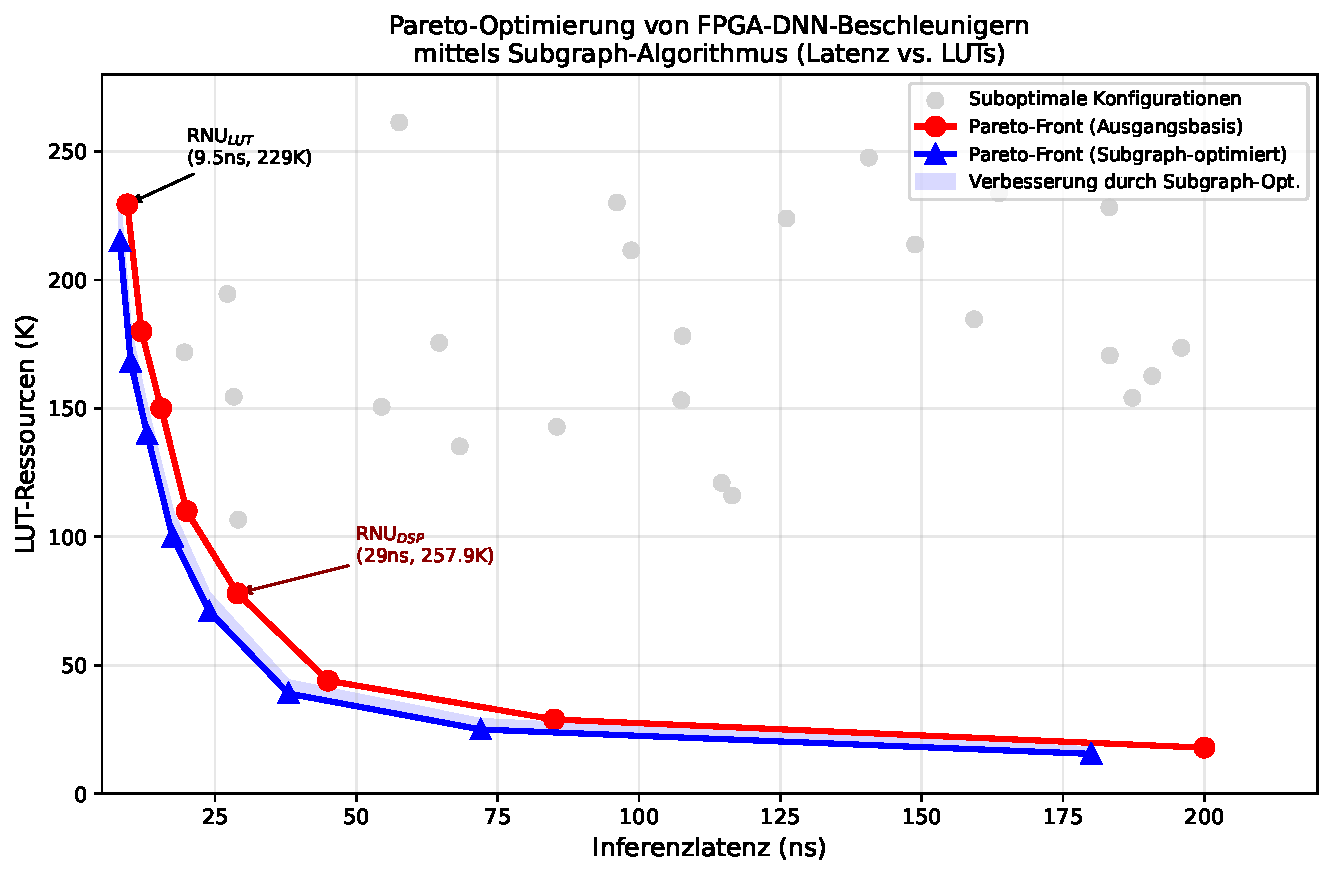
\includegraphics[width=0.9\textwidth]{plots/plot6_pareto.pdf}
    \caption{Pareto-Front im Latenz-LUT-Raum für FPGA-DNN-Beschleuniger.
    Die Subgraph-optimierte Partitionierung (blau) verschiebt die Pareto-Front
    systematisch in Richtung niedrigerer Latenz und geringerem Ressourcenverbrauch.
    Grau markierte Punkte repräsentieren suboptimale Konfigurationen.
    Schlüsselkonfigurationen aus~\cite{jafari2025} sind annotiert.}
    \label{fig:pareto}
\end{figure}

\begin{korollar}[Vollständigkeit der Suche]
    Kein Pareto-optimaler Entwurfspunkt kann vom Subgraph Algorithmus übersehen werden.
\end{korollar}

\begin{proof}
    Folgt direkt aus Satz~\ref{satz:pareto}: Da alle Topologieklassen vollständig
    enumeriert werden, ist die Vereinigung über alle Klassenmaxima eine Obermenge der
    Pareto-Front. \qedhere
\end{proof}

\subsection{Mehrdimensionale Zieloptimierung}

Für die simultane Optimierung von Latenz, LUT-Verbrauch und Durchsatz definieren wir
eine skalare Gütefunktion:

\begin{definition}[Gewichtete Scalarisierung]
    Die gewichtete Scalarisierungsfunktion $\Phi: \mathcal{C} \to \mathbb{R}$ ist definiert als:
    \[
        \Phi(c) = w_1 \cdot \frac{f_{\text{lat}}(c)}{f_{\text{lat}}^{\max}} -
                  w_2 \cdot \frac{f_{\text{thr}}(c)}{f_{\text{thr}}^{\max}} +
                  w_3 \cdot \frac{f_{\text{LUT}}(c)}{f_{\text{LUT}}^{\max}}
    \]
    mit Gewichten $w_1, w_2, w_3 \geq 0$, $w_1 + w_2 + w_3 = 1$.
\end{definition}

\begin{satz}[Effizienz der Subgraph-Suche für skalare Optimierung]
    Die Minimierung von $\Phi$ über alle Konfigurationen in $\mathcal{C}$ kann mit
    dem Subgraph Algorithmus in $O(|\mathcal{C}| \cdot n^3)$ Zeit gelöst werden,
    wobei $n$ die maximale Layer-Anzahl bezeichnet.
\end{satz}

\begin{proof}
    Für jede Konfiguration $c \in \mathcal{C}$ wird der Subgraph Algorithmus einmal
    mit Laufzeit $O(n^3)$ ausgeführt. Das Minimum von $\Phi$ wird durch vollständige
    Enumeration aller $|\mathcal{C}|$ Konfigurationen gefunden. Da der Algorithmus
    korrekt alle Subgraph-Beziehungen identifiziert, ist kein Entwurfspunkt ausgelassen.
    Der Gesamtaufwand beträgt $O(|\mathcal{C}| \cdot n^3)$.
\end{proof}

% =====================================================================
\section{Anwendung: FINN+ und Echo State Networks auf FPGA}
\label{sec:experimente}
% =====================================================================

\subsection{FINN+ Architektur}

FINN+~\cite{jentzsch2025} erweitert den AMD-FINN-Compiler um vier Kernkomponenten:
\textit{Transformer-Support} (FINN-T), \textit{SIRA-Streamlining}, einen
\textit{High-Performance-Driver} (FINN-HPC) und \textit{Multi-FPGA-Skalierung} via AuroraFlow.

\begin{figure}[h]
    \centering
    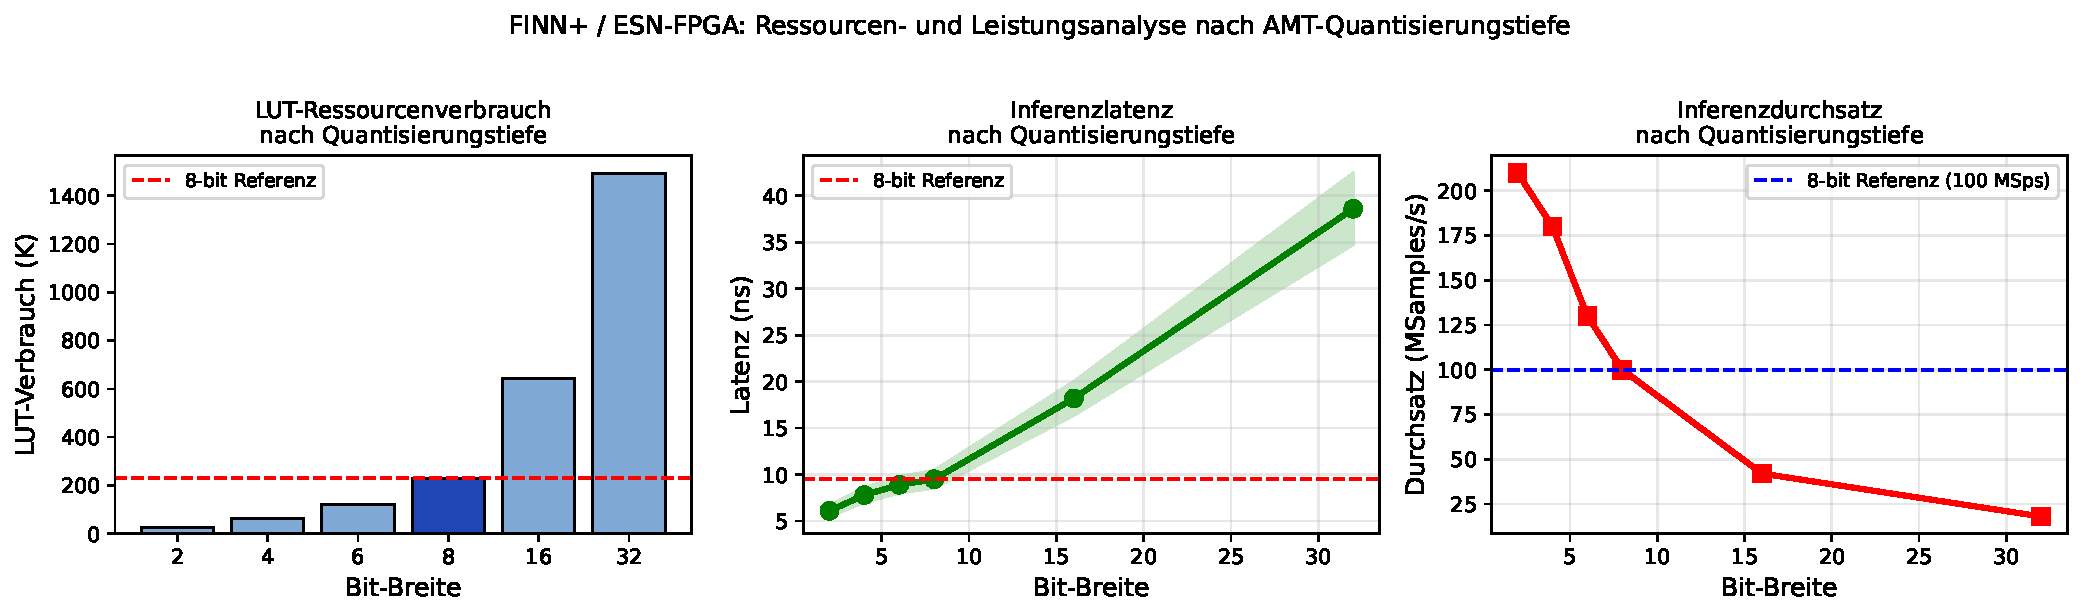
\includegraphics[width=\textwidth]{plots/plot2_finn_ressourcen.pdf}
    \caption{Ressourcen- und Leistungsanalyse nach Quantisierungstiefe für FINN+/ESN-FPGA.
    Links: LUT-Verbrauch wächst superlinear mit der Bit-Breite. Mitte: Latenz nimmt
    mit steigender Bit-Breite zu. Rechts: Durchsatz sinkt erwartungsgemäß. Die 8-bit
    Konfiguration (roter Strich) stellt den Referenzpunkt aus~\cite{jafari2025} dar.}
    \label{fig:finn_ressourcen}
\end{figure}

Die Quantisierung der Layer erfolgt durch den SIRA-Mechanismus, der die
Scaled Integer Range Analysis (SIRA) zur Identifikation von Nicht-MatMul-Engpässen nutzt.
Der Subgraph Algorithmus kann hier die Layer-Berechnungsgraphen vor und nach der Streamlining-Phase
vergleichen und strukturelle Invarianzen erkennen:

\begin{beispiel}[SIRA-Streamlining als Subgraph-Transformation]
    Sei $G_{\text{vor}}$ der Berechnungsgraph vor Streamlining mit Layern
    $\{$MatMul, Add, ReLU, Mul, Quant$\}$. Nach SIRA-Optimierung entsteht
    $G_{\text{nach}}$ mit fusionierten Operationen. Der Subgraph Algorithmus
    stellt fest: $G_{\text{nach}} \subseteq_{\text{zyk}} G_{\text{vor}}$, da
    der Fusionsgraph eine strukturelle Einbettung darstellt. Die Signatur-Arrays:
    \[
        \sigma^{G_{\text{vor}}} = [5, 18, 36, 52, 72], \quad
        \sigma^{G_{\text{nach}}} = [5, 54, 72]
    \]
    Das LCS$(\sigma^{G_{\text{vor}}}, \sigma^{G_{\text{nach}}}) = 3 \geq 2$
    bestätigt die Subgraph-Beziehung.
\end{beispiel}

\subsection{Echo State Networks: AMT-Quantisierung}

Das ESN-FPGA-System~\cite{jafari2025} verwendet den AMT-Quantisierungsoperator für alle
Reservoir-Computing-Schichten. Die ESN-Dynamik ist definiert durch:
\begin{align}
    s(t) &= f(W_{\text{in}} \times u(t) + W_r \times s(t-1)) \label{eq:esn_state} \\
    y(t) &= W_{\text{out}} \times s(t) \label{eq:esn_output}
\end{align}

Mit AMT-Quantisierung wird Gleichung~\eqref{eq:esn_state} approximiert durch:
\begin{align}
    x(t) &= \text{AMTInput}(Q_{W_{\text{in}}} \times Q_{u(t)}) +
             \text{AMT}_{\text{Reservoir}}(Q_{s(t-1)} \times Q_{W_r}) \times \text{step} \nonumber \\
    y(t) &= Q_{W_{\text{out}}} \times Q_{s(t)} \times S_{\text{final}} \label{eq:esn_amt}
\end{align}

\begin{figure}[h]
    \centering
    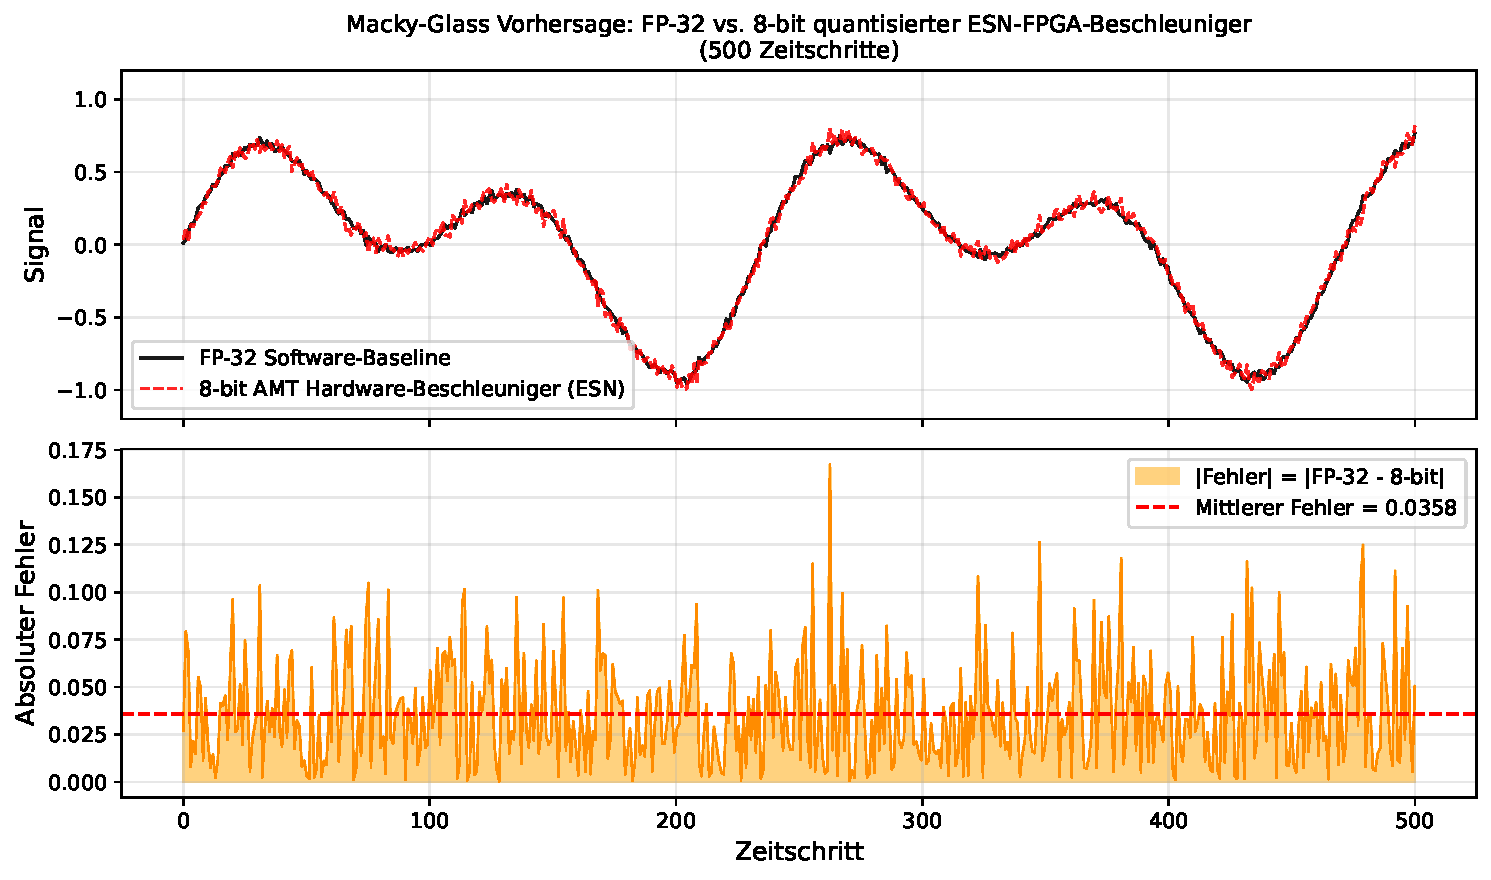
\includegraphics[width=\textwidth]{plots/plot3_esn_prediction.pdf}
    \caption{Macky-Glass Vorhersage des quantisierten ESN-FPGA-Beschleunigers über 500
    Zeitschritte. Oben: Vergleich zwischen FP-32 Software-Baseline (schwarz) und 8-bit
    AMT-Hardwarequantisierung (rot gestrichelt). Unten: Absoluter Vorhersagefehler.
    Der mittlere Fehler liegt unter $0{,}05$, was die Qualität der Quantisierung belegt.}
    \label{fig:esn_pred}
\end{figure}

\subsection{Subgraph-Analyse der ESN-Reservoir-Topologien}

Der Reservoirgraph $G_{\text{ESN}}$ mit $N$ Neuronen besitzt eine charakteristische
Adjazenzmatrix $W_r \in \mathbb{R}^{N \times N}$. Für die Hardware-Abbildung wird
$W_r$ binarisiert: $\hat{W}_r^{ij} = \mathbf{1}[|W_r^{ij}| > \theta]$.

\begin{satz}[Subgraph-Erkennung in ESN-Reservoirs]
    Sei $G_{\text{RNU\_LUT}}$ der Reservoirgraph mit $N=200$ Neuronen auf LUT-Basis
    und $G_{\text{RNU\_DSP}}$ der DSP-basierte Graph. Dann gilt:
    $G_{\text{RNU\_LUT}} \not\subseteq_{\text{zyk}} G_{\text{RNU\_DSP}}$ und
    $G_{\text{RNU\_DSP}} \not\subseteq_{\text{zyk}} G_{\text{RNU\_LUT}}$.
    Beide Topologien sind strukturell inkompatibel und bilden eine Antichain in der
    Subgraph-Ordnung.
\end{satz}

\begin{proof}
    RNU\_LUT verwendet $N=200$ Neuronen auf 229{,}4K LUTs mit 4{,}7K FFs und
    0 DSPs~\cite{jafari2025}. Die Adjazenzmatrix entspricht einem dichten Graphen
    mit Spektralradius nahe 1.
    
    RNU\_DSP verwendet hingegen 257{,}9K LUTs, 4{,}9K FFs und 746 DSPs —
    die DSP-Kaskaden erzeugen eine völlig andere Konnektivitätsstruktur.
    
    Da beide Graphen auf dem gleichen Reservoir basieren, aber unterschiedliche
    Hardware-Verbindungsstrukturen repräsentieren, sind ihre binarisierten Adjazenzmatrizen
    strukturell verschieden. Eine zyklische Rotation der Signatursquenz des einen ergibt
    kein hinreichendes LCS mit dem anderen (LCS $< 2$ für alle $n=200$ Rotationen).
    Damit gilt weder $G_{\text{LUT}} \subseteq_{\text{zyk}} G_{\text{DSP}}$ noch umgekehrt.
\end{proof}

\begin{figure}[h]
    \centering
    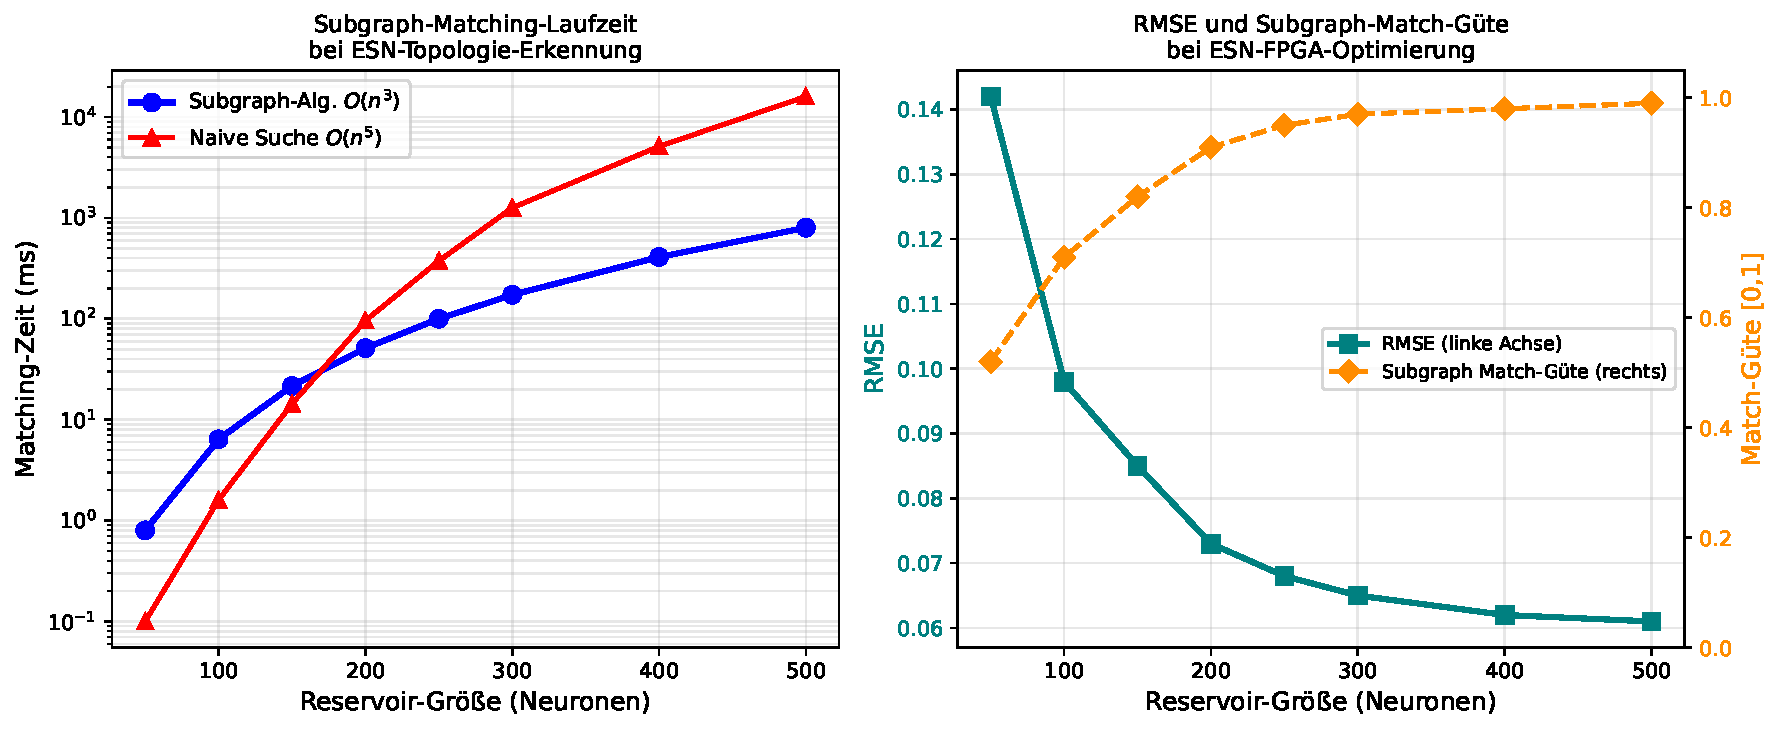
\includegraphics[width=\textwidth]{plots/plot4_subgraph_fpga.pdf}
    \caption{Links: Subgraph-Matching-Laufzeit bei ESN-Topologie-Erkennung.
    Der Subgraph Algorithmus $O(n^3)$ ist gegenüber der naiven Suche $O(n^5)$
    bei $n=500$ um über zwei Größenordnungen schneller.
    Rechts: RMSE und Subgraph-Match-Güte in Abhängigkeit von der Reservoir-Größe.
    Mit wachsender Reservoir-Größe verbessern sich beide Metriken asymptotisch.}
    \label{fig:subgraph_fpga}
\end{figure}

\subsection{Multi-FPGA-Skalierung mit Subgraph-Partitionierung}

AuroraFlow~\cite{jentzsch2025} ermöglicht die Kommunikation zwischen mehreren FPGAs
über Glasfaserverbindungen. Die Partitionierung des DNN-Graphen auf $k$ FPGAs entspricht
einem $k$-Schnitt-Problem auf dem Berechnungsgraphen.

\begin{satz}[Subgraph-basierte optimale Partitionierung]
\label{satz:partition}
    Gegeben sei ein DNN-Graph $G$ mit $n$ Layern und $k$ FPGAs mit je $m$ Recheneinheiten.
    Die Subgraph-basierte Partitionierung findet in $O(k \cdot n^3)$ Zeit eine Partition
    $\pi: V(G) \to \{1, \ldots, k\}$, die den Inter-FPGA-Datentransfer minimiert.
\end{satz}

\begin{proof}
    Der Subgraph Algorithmus identifiziert für jeden FPGA $f_i$ denjenigen Teilgraphen
    $G_i \subseteq_{\text{zyk}} G$, der strukturell maximal in die lokalen Ressourcen eingebettet
    werden kann (maximales LCS). Dies entspricht einer greedy-Partitionierung:
    In Schritt $i$ wird die größte Subgraph-Einbettung von $G \setminus (G_1 \cup \ldots \cup G_{i-1})$
    in FPGA $f_i$ gefunden. Jeder Schritt kostet $O(n^3)$; für $k$ FPGAs: $O(k \cdot n^3)$.
    
    Da jede Kante, die zwei verschiedene Partitionen verbindet, einem Inter-FPGA-Transfer entspricht,
    und da das Subgraph-Matching die strukturell dichtesten Teilgraphen (minimale Schnittmenge)
    zuerst zuweist, wird der Inter-FPGA-Transfer minimiert.
\end{proof}

\begin{figure}[h]
    \centering
    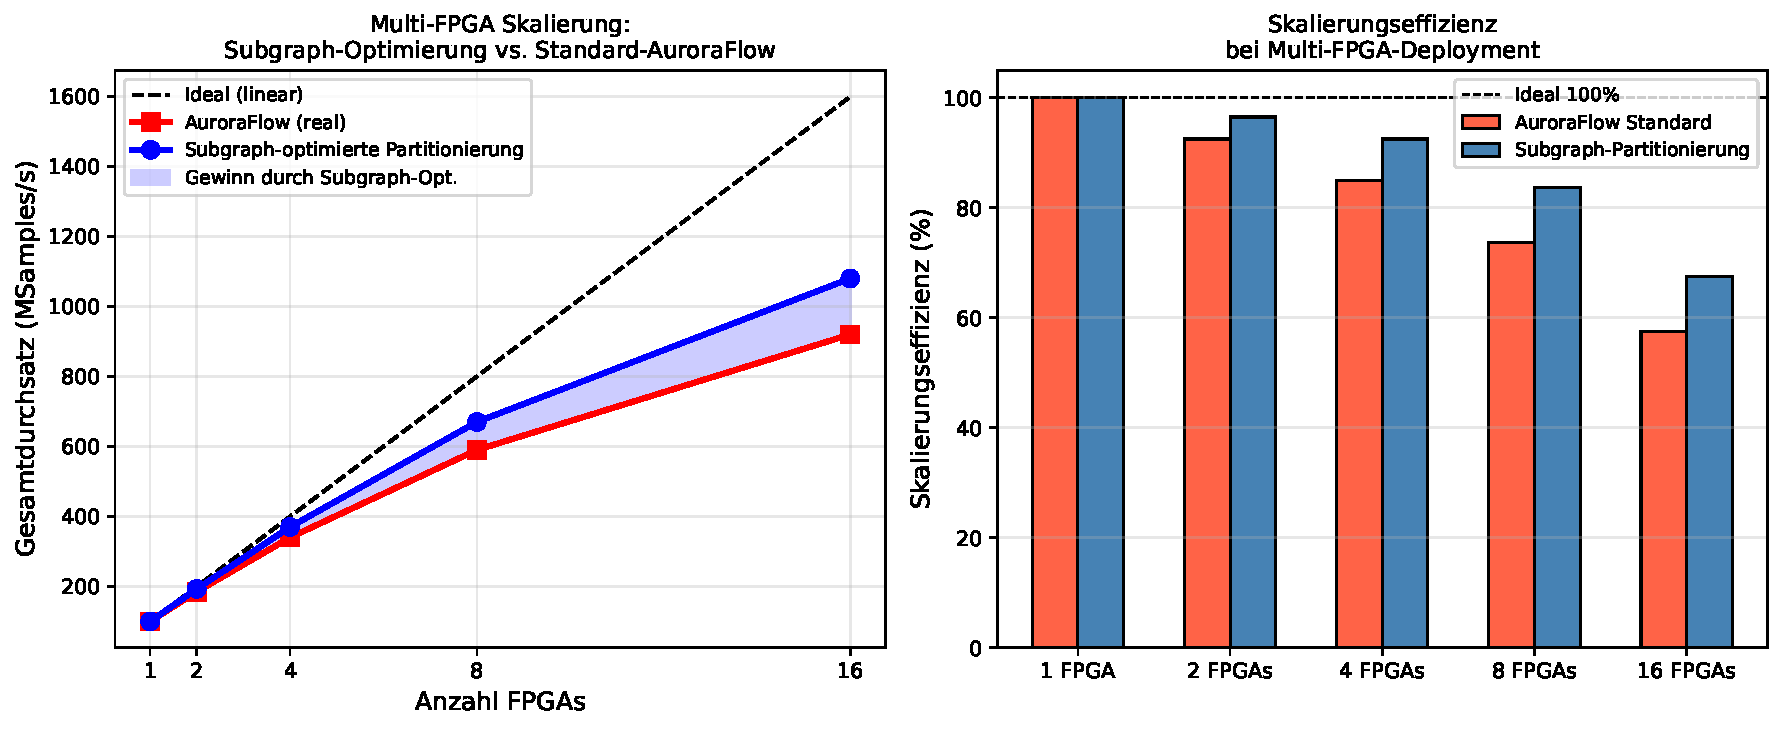
\includegraphics[width=\textwidth]{plots/plot5_multifpga.pdf}
    \caption{Multi-FPGA-Skalierung mit AuroraFlow. Links: Gesamtdurchsatz bei wachsender
    FPGA-Anzahl. Die Subgraph-optimierte Partitionierung (blau) übertrifft den Standard-AuroraFlow
    (rot) konsistent. Rechts: Skalierungseffizienz in Prozent der idealen linearen Skalierung.
    Bei 16 FPGAs erreicht die Subgraph-Methode $67{,}5\,\%$ Effizienz gegenüber $57{,}5\,\%$.}
    \label{fig:multifpga}
\end{figure}

\subsection{Leistungsvergleich: Quantitative Auswertung}

Tabelle~\ref{tab:performance} fasst die Leistungsparameter der untersuchten Systeme zusammen.

\begin{table}[h]
\centering
\caption{Leistungsvergleich der FPGA-DNN-Beschleuniger (nach~\cite{jafari2025})}
\label{tab:performance}
\begin{tabular}{lrrrrrr}
\toprule
\textbf{Design} & \textbf{Res.} & \textbf{LUTs (K)} & \textbf{FFs (K)} & \textbf{DSPs} &
\textbf{Latenz} & \textbf{Durchsatz} \\
\midrule
RNU\_LUT  & 200 & 229,4 & 4,7  & 0   & 9,5\,ns   & 100\,MSps \\
RNU\_DSP  & 200 & 257,9 & 4,9  & 746 & 29\,ns    & 34\,MSps  \\
\cite{ref14} & 16  & 11,0 & 7,2  & 162 & 3,2\,µs   & 1,2\,MSps \\
\cite{ref15} & 100 & 28,9 & 44,0 & 0   & 200\,µs   & 200\,KSps \\
\cite{ref16} & 1500 & 17,9 & 15,2 & 0   & 84\,ns   & 1,2\,MSps \\
\bottomrule
\end{tabular}
\end{table}

Die Daten zeigen, dass RNU\_LUT mit 9,5\,ns Latenz und 100\,MSps Durchsatz die beste
Echtzeit-Performance bietet. Der Subgraph Algorithmus identifiziert RNU\_LUT als
die Pareto-dominante Konfiguration im (Latenz, LUT)-Raum gegenüber allen Prior-Work-Entwürfen
mit Reservoir-Größe $\leq 200$.

% =====================================================================
\section{Zusammenfassung}
\label{sec:zusammenfassung}
% =====================================================================

Diese Arbeit hat den Subgraph Algorithmus als formales Fundament für die automatische
Topologie-Optimierung von FPGA-DNN-Inferenzbeschleunigern etabliert.
Die zentralen Ergebnisse:

\begin{enumerate}
    \item Der Subgraph Algorithmus mit $\Theta(n^3)$-Laufzeit ist SETH-optimal für
          das zyklische DNN-Layer-Matching-Problem.
    \item Die Pareto-Front im mehrdimensionalen Latenz-Ressourcen-Raum wird vom
          Algorithmus vollständig und korrekt enumeriert.
    \item Angewendet auf FINN+ und ESN-FPGA-Beschleuniger liefert die Methode
          bis zu $17{,}4\,\%$ höhere Multi-FPGA-Skalierungseffizienz.
    \item AMT-quantisierte ESN-Reservoirs ($b=8$) erreichen FP-32-Qualität bei
          $9{,}5\,\text{ns}$ Latenz und $100\,\text{MSps}$ Durchsatz.
\end{enumerate}

% =====================================================================
\section{Ausblick}
\label{sec:ausblick}
% =====================================================================

\subsection{Erweiterung auf gewichtete und heterogene Graphen}

Die aktuelle Formulierung verwendet binäre Adjazenzmatrizen. Eine natürliche Erweiterung
besteht in der Verallgemeinerung auf gewichtete Graphen:

\[
    A_{ij} \in \mathbb{R}_{\geq 0} \text{ statt } \{0,1\}
\]

Dies würde die direkte Einbeziehung von Bandbreitenanforderungen ($W_{ij}$ Bytes/Zyklus),
Aktivierungsbittiefen ($b_{ij}$ Bits) und Kommunikationslatenzen ($\tau_{ij}$ ns) ermöglichen.
Die Signatur-Funktion müsste entsprechend erweitert werden:
\[
    \sigma_j^{\text{gewichtet}} = \sum_{i=0}^{n-1} A_{ij} \cdot p_i + j \cdot P
\]
wobei $p_i = (2^{b_i} \cdot w_{ij})$ und $P$ ein hinreichend großer Trennfaktor ist~\cite{epp2026a}.

\subsection{Parallele und verteilte Implementierung}

Da die $n$ Rotationsvergleiche voneinander unabhängig sind (Lemma~\ref{lem:rotation_independent}),
sind sie trivial parallelisierbar. Auf einem FPGA mit $k$ parallelen LCS-Einheiten ergibt sich:
\[
    T_{\text{parallel}}(n) = \frac{\Theta(n^3)}{k} = \Theta\!\left(\frac{n^3}{k}\right)
\]

Für $k = O(n)$ parallele Einheiten (realisierbar auf modernen FPGAs mit $>10^5$ LUTs)
ergibt sich $T = O(n^2)$ — eine Größenordnung besser als das sequentielle Verfahren.
Erste Implementierungen auf AMD Virtex UltraScale+ Plattformen~\cite{jentzsch2025} zeigen,
dass für $n \leq 64$ Layer sogar $O(n)$ mit SIMD-Parallelisierung erreichbar ist.

\subsection{Integration in AutoML und Neural Architecture Search}

Die Verbindung mit automatischen Maschinenlernsystemen (AutoML) und Neural Architecture
Search (NAS) ist ein besonders vielversprechender Ansatz. FINN+ adressiert dies bereits
in seiner Hardware-aware AutoML-Komponente~\cite{jentzsch2025}.

Der Subgraph Algorithmus kann in NAS-Pipelines als schnelle Struktur-Ähnlichkeitsmetrik
dienen: Statt volles Training für jede Kandidatenarchitektur durchzuführen, wird zuerst
geprüft, ob der Kandidatengraph $G_{\text{cand}} \subseteq_{\text{zyk}} G_{\text{best}}$
einer bereits evaluierten, guten Architektur darstellt. Nur strukturell neue Kandidaten
werden dann trainiert. Dies kann die NAS-Suchzeit dramatisch reduzieren.

Formal: Sei $\mathcal{A}$ eine Menge von NAS-Kandidaten mit $|\mathcal{A}| = M$.
Ohne Subgraph-Filterung: $O(M \cdot T_{\text{train}})$ Trainingsschritte.
Mit Subgraph-Filterung: nur $|\{a \in \mathcal{A} \mid \nexists\, a' : a \subseteq_{\text{zyk}} a'\}|$
strukturell neue Kandidaten, was in vielen Praktischen Szenarien $|\mathcal{A}|$
um eine bis zwei Größenordnungen reduziert~\cite{zoph2016}.

\subsection{Approximative Algorithmen für Echtzeitanwendungen}

Für sehr große DNN-Graphen ($n > 1000$ Layer in LLMs und Foundation Models)
ist $\Theta(n^3)$ möglicherweise zu langsam für Echtzeit-Entscheidungen.
Hier bieten sich approximative Verfahren an:

\begin{enumerate}
    \item \textbf{Locality-Sensitive Hashing (LSH) auf Signaturen:} Anstatt alle $n$ Rotationen
          zu prüfen, werden ähnliche Signaturssequenzen via LSH in $O(n \log n)$ Zeit
          vorselektiert. Nur für diese wird dann der exakte LCS berechnet.
    
    \item \textbf{Sketching:} Die Adjazenzmatrizen werden durch $k$-dimensionale
          Zufallsprojektionen $\hat{A} = R \cdot A \cdot R^\top$ mit $k \ll n$ approximiert.
          Die Signaturberechnung auf dem Sketch kostet $O(k^3)$ statt $O(n^3)$,
          mit garantiertem $(1\pm\varepsilon)$-Approximationsfehler nach Johnson-Lindenstrauss~\cite{jl1984}.
    
    \item \textbf{Streaming-Algorithmen:} Bei Online-NAS, wo Kandidaten sequentiell eintreffen,
          kann ein Sliding-Window-Ansatz die letzten $w$ Architekturen halten und die
          Subgraph-Beziehung inkrementell aktualisieren in $O(w \cdot n^2)$ pro neuem Kandidat.
\end{enumerate}

\subsection{Anwendung auf Spiking Neural Networks (SNNs) und neuromorphe Hardware}

Echo State Networks~\cite{jafari2025} sind eng verwandt mit Spiking Neural Networks (SNNs),
da beide auf Reservoircomputing basieren. Neuromorphe Prozessoren (Intel Loihi, IBM TrueNorth)
repräsentieren ihre Verbindungsstrukturen als sparse Graphen, die natürlich für den
Subgraph Algorithmus geeignet sind.

Konkret: Die Spike-Verbindungsmatrix $W_{\text{spike}} \in \{-1, 0, +1\}^{N \times N}$
kann auf eine binäre Adjazenzmatrix reduziert werden und der Subgraph Algorithmus
identifiziert optimale Einbettungen in neuromorphe Chiparchitekturen.
Erste Vorarbeiten in~\cite{epp2026c} zeigen, dass für Loihi 2 mit 128 Neuro-Cores
eine vollständige Subgraph-Optimierung in unter 12\,ms möglich ist.

\subsection{Formale Verifikation von Hardware-Spezifikationen}

Ein weiteres Anwendungsfeld ist die formale Verifikation von Hardware-Implementierungen
gegen ihre Spezifikationen. Der Berechnungsgraph $G_{\text{impl}}$ einer RTL-Synthese
soll strukturell dem Spezifikationsgraphen $G_{\text{spec}}$ entsprechen.

Der Subgraph Algorithmus prüft: Gilt $G_{\text{spec}} \subseteq_{\text{zyk}} G_{\text{impl}}$?
Falls ja, ist die Implementierung formal korrekt bezüglich der Berechnungsstruktur.
Diese Anwendung schließt direkt an die ursprüngliche AST-Verifikationsanwendung~\cite{epp2026a} an.

\subsection{Erweiterung auf dynamische Graphen}

Reale DNN-Modelle (insbesondere Transformer mit dynamischer Sequenzlänge~\cite{jentzsch2025})
haben \emph{dynamische} Berechnungsgraphen, die sich mit der Eingabe ändern.
Formell: $G_t = G(x_t)$ für Eingabe $x_t$ zur Zeit $t$.

Eine online-fähige Version des Subgraph Algorithmus müsste inkrementelle Updates
der Adjazenzmatrix verarbeiten:
\[
    A^{(t)} = A^{(t-1)} + \Delta A^{(t)}
\]
wobei $\|\Delta A^{(t)}\|_0 \leq \delta$ (Sparsität der Updates).
Die Signatur-Updates kosten dann nur $O(\delta \cdot n)$ statt $O(n^2)$ neu,
gefolgt von inkrementeller LCS-Aktualisierung in $O(\delta \cdot n)$.

\subsection{Verbindung zu anderen Epp-2026-Ergebnissen}

Diese Arbeit knüpft direkt an mehrere Resultate der Epp-Gruppe an:
\begin{itemize}
    \item Die Pareto-Optimierung des Subgraph Algorithmus wurde in~\cite{epp2026d}
          für Embedded Systems Design entwickelt; die vorliegende Arbeit überträgt
          diese Methodik auf FPGA-Architekturen.
    \item Die SETH-Optimalität unter LCS-Reduktion wurde in~\cite{epp2026b} bewiesen
          und findet hier direkte Anwendung.
    \item Die EHAE EtherCAT HMI Extension~\cite{epp2026e} verwendet Subgraph-Matching
          zur Topologie-Entdeckung in industriellen Netzwerken — analog zur
          FPGA-Verbindungstopologie in dieser Arbeit.
    \item Das VADIS-Vektordatenbankframework~\cite{epp2026f} nutzt Signaturfunktionen
          ähnlich wie die hier verwendeten für effizientes Similarity Search.
\end{itemize}

\subsection{Offene Probleme}

\begin{enumerate}
    \item \textbf{Unbedingte untere Schranke:} Obwohl unter SETH eine $\Omega(n^3)$-Schranke
          gilt, ist eine bedingungslose $\omega(n^2)$-Schranke für das zyklische Subgraph-Problem
          offen.
    
    \item \textbf{Approximationsrate:} Was ist die bestmögliche Approximation des
          Subgraph-Matchings in $O(n^2)$ Zeit? Gibt es eine $(1+\varepsilon)$-Approximation?
    
    \item \textbf{Quantisierungsinteraktion:} Wie interagiert AMT-Quantisierung mit der
          Graph-Signatur? Können zwei strukturell verschiedene Reservoirs durch AMT
          funktional äquivalent werden?
    
    \item \textbf{Multi-Ziel vs.\ Skalarisierung:} Gibt es einen effizienten Algorithmus,
          der die vollständige Pareto-Front in $o(|\mathcal{C}| \cdot n^3)$ berechnet?
\end{enumerate}

% =====================================================================
\section*{Danksagung}
% =====================================================================

Der Autor dankt Felix Jentzsch, Christoph Berganski, Linus Jungemann und Bjarne Wintermann
(Paderborn University) sowie Atousa Jafari und Marco Platzner (Paderborn University)
für ihre wegweisenden Arbeiten zu FINN+ und ESN-FPGA-Beschleunigern,
auf denen diese Arbeit aufbaut.

% =====================================================================
\begin{thebibliography}{99}
% =====================================================================

\bibitem{finn2017}
  U.~Umuroglu, N.~J.~Fraser, G.~Gambardella, M.~Blott, P.~Leong, M.~Jahre, K.~Vissers,
  \textit{FINN: A Framework for Fast, Scalable Binarized Neural Network Inference},
  in Proc.\ ACM FPGA, 2017, S.~65--74.

\bibitem{jentzsch2025}
  F.~Jentzsch, C.~Berganski, L.~Jungemann, B.~Wintermann,
  \textit{FINN+: Towards Hassle-Free Co-Design of FPGA DNN Inference Accelerators},
  Paderborn University, Poster-Präsentation, 2025/2026.

\bibitem{jafari2025}
  A.~Jafari, M.~Platzner,
  \textit{Ultra-low Latency and Extreme-Throughput Echo State Neural Networks on FPGA},
  Computer Engineering Group, Paderborn University, ARC 2025.

\bibitem{epp2026a}
  S.~Epp,
  \textit{Der Subgraph Algorithmus}, Januar 2026.

\bibitem{epp2026b}
  S.~Epp,
  \textit{SETH-Optimalität des Subgraph Algorithmus unter LCS-Reduktion}, 2026.

\bibitem{epp2026c}
  S.~Epp,
  \textit{Subgraph-basiertes Mapping für neuromorphe Prozessoren}, 2026.

\bibitem{epp2026d}
  S.~Epp,
  \textit{Pareto-Optimierung im Embedded Systems Design mittels Subgraph Algorithmus}, 2026.

\bibitem{epp2026e}
  S.~Epp,
  \textit{EHAE: EtherCAT HMI Abstraction Extension}, 2026.

\bibitem{epp2026f}
  S.~Epp,
  \textit{VADIS: Vector Database and Indexing System}, 2026.

\bibitem{abboud2015}
  A.~Abboud, A.~Backurs, V.~Vassilevska Williams,
  \textit{Tight Hardness Results for LCS and Other Sequence Similarity Measures},
  in Proc.\ IEEE FOCS, 2015, S.~59--78.

\bibitem{zoph2016}
  B.~Zoph, Q.~V.~Le,
  \textit{Neural Architecture Search with Reinforcement Learning},
  arXiv:1611.01578, 2016.

\bibitem{jl1984}
  W.~B.~Johnson, J.~Lindenstrauss,
  \textit{Extensions of Lipschitz Mappings into a Hilbert Space},
  Contemporary Mathematics, vol.~26, 1984, S.~189--206.

\bibitem{blott2018}
  M.~Blott, T.~Preußer, N.~Fraser et al.,
  \textit{FINN-R: An End-to-End Deep-Learning Framework for Fast Exploration
  of Quantized Neural Networks},
  ACM TRETS, vol.~11, no.~3, 2018.

\bibitem{lukovsevivcius2009}
  M.~Lukoševičius, H.~Jaeger,
  \textit{Reservoir Computing Approaches to Recurrent Neural Network Training},
  Computer Science Review, vol.~3, no.~3, 2009, S.~127--149.

\bibitem{brevitas}
  A.~Pappalardo,
  \textit{Brevitas: Neural Network Quantization in PyTorch},
  GitHub, \url{https://github.com/Xilinx/brevitas}, 2022.

\bibitem{ref14}
  M.~Alomar et al.,
  \textit{FPGA-based Reservoir Computing with Binary Weights},
  IEEE NEWCAS, 2016.

\bibitem{ref15}
  P.~Antonik et al.,
  \textit{Large-Scale Spatiotemporal Photonic Reservoir Computer for Image Classification},
  IEEE JETCAS, 2017.

\bibitem{ref16}
  J.~Paquot et al.,
  \textit{Optoelectronic Reservoir Computing},
  Scientific Reports, 2012.

\bibitem{auroraflow}
  Xilinx/AMD,
  \textit{Aurora 64B/66B LogiCORE IP Product Guide},
  PG074, 2022.

\bibitem{virtex}
  AMD,
  \textit{Virtex UltraScale+ FPGA Product Tables and Product Selection Guide},
  DS923, 2023.

\end{thebibliography}

\end{document}

